\documentclass[a4paper,10pt]{article}
\usepackage[utf8]{inputenc}
\usepackage{ngerman}
\usepackage{eurosym}
\usepackage{algorithm2e}
%\usepackage{ stmaryrd }
\usepackage{enumerate}
\usepackage{tikz}
\usetikzlibrary{trees,automata,arrows,shapes}
\usepackage{graphicx}
\usepackage{listings}
\usepackage{xcolor}
\usepackage{amsmath, amsthm}
\usepackage{listings}
\usepackage{amsfonts, amssymb}
\usepackage{algorithm2e}
\usepackage{textcomp}
\usepackage{bussproofs}
\usepackage{rotating}
\usepackage{caption}
\usepackage{listings}% http://ctan.org/pkg/listings
\lstset{
  basicstyle=\ttfamily,
  mathescape
}
\renewcommand*{\proofname}{Beweis}

%opening
\title{}
\author{}

\begin{document}
\noindent Thomas Stüber (3750920) \hfill Tübingen, den  \today\\
\noindent Benjamin Coban (3526251) \\
\begin{center}
\Large Übungen zur Vorlesung  \\ ``SAT-Solving und Anwendungen'' \\
\vspace*{2mm}
\large (Abgabe 7) \\
\vspace*{2mm}
\end{center}

\noindent\textbf{Aufgabe 7.1}\\

Gegeben sei folgende Aussage in non-CNF:
\begin{align*}
F = (z \wedge x) \vee \neg(\neg x \wedge y)
\end{align*}
mit seinem zugehörigen DAG. Es ist der nonCNF-Algorithmus aus der Vorlesung anzuwenden, um eine mögliche Belegung der Formel $F$ zu finden. Dabei entsteht folgende Tabelle:\\
\begin{tabular}{|c|c|c|c|c|c|c|}
	\hline 
	lvl & var & val & Reason & Clause & Stack & Comment \\ 
	\hline 
	1 & $\vee$ & T & Decision & - & $\vee=T@1$ & root init \\ 
	\hline 
	2 & $\neg_0$ & F & Decision & - & $\neg_0=F@2$ & negate first \\ 
	\hline 
	& $\wedge_1$ & T & Parent & $\neg_0=F$ & $\wedge_1=T@2$ &  \\ 
	\hline 
	& $\wedge_0$ & T & Parent & $\neg_0=F,\vee = T$ & $\wedge_0=T@2$ &  \\ 
	\hline 
	& $\neg_1$ & T & Parent & $\wedge_1=T$ & $\neg_1=T@2$ &  \\ 
	\hline 
	& $x$ & T & Parent & $\wedge_0=T$ & $x=T@2$ & \textcolor{red}{Conflict} \\ 
	\hline 
	& $x$ & F & Parent & $\neg_1=T$ & $x=F@2$ & \textcolor{red}{Conflict} \\ 
	\hline 
\end{tabular}\\\\Nun ist ein Konflikt gegeben, welcher im folgenden Implikationsgraph illustriert wird:

\begin{center}
	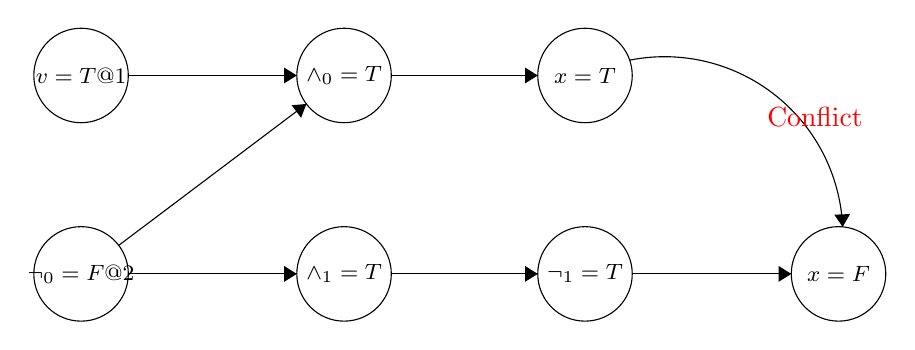
\begin{tikzpicture}[scale=0.2]
	\tikzstyle{every node}+=[inner sep=0pt]
	\draw [black] (10.3,-11.7) circle (3);
	\draw (10.3,-11.7) node {\smaller$v=T@1$};
	\draw [black] (27,-11.7) circle (3);
	\draw (27,-11.7) node {\smaller$\wedge_0=T$};
	\draw [black] (42.3,-11.7) circle (3);
	\draw (42.3,-11.7) node {\smaller$x=T$};
	\draw [black] (42.3,-24.3) circle (3);
	\draw (42.3,-24.3) node {\smaller$\neg_1=T$};
	\draw [black] (27,-24.3) circle (3);
	\draw (27,-24.3) node {\smaller$\wedge_1=T$};
	\draw [black] (10.3,-24.3) circle (3);
	\draw (10.3,-24.3) node {\smaller$\neg_0=F@2$};
	\draw [black] (58.4,-24.3) circle (3);
	\draw (58.4,-24.3) node {\smaller$x=F$};
	\draw [black] (13.3,-11.7) -- (24,-11.7);
	\fill [black] (24,-11.7) -- (23.2,-11.2) -- (23.2,-12.2);
	\draw [black] (12.69,-22.49) -- (24.61,-13.51);
	\fill [black] (24.61,-13.51) -- (23.67,-13.59) -- (24.27,-14.39);
	\draw [black] (13.3,-24.3) -- (24,-24.3);
	\fill [black] (24,-24.3) -- (23.2,-23.8) -- (23.2,-24.8);
	\draw [black] (30,-11.7) -- (39.3,-11.7);
	\fill [black] (39.3,-11.7) -- (38.5,-11.2) -- (38.5,-12.2);
	\draw [black] (30,-24.3) -- (39.3,-24.3);
	\fill [black] (39.3,-24.3) -- (38.5,-23.8) -- (38.5,-24.8);
	\draw [black] (45.3,-24.3) -- (55.4,-24.3);
	\fill [black] (55.4,-24.3) -- (54.6,-23.8) -- (54.6,-24.8);
	\draw [black] (45.129,-10.729) arc (101.34918:2.55673:11.318);
	\fill [black] (58.66,-21.32) -- (59.13,-20.5) -- (58.13,-20.54);
	\draw (56.9,-14.97) node [above] {\textcolor{red}{Conflict}};
	\end{tikzpicture}
\end{center}
Auf den Kanten steht jeweils \underline{Parent als Reason}. Es entsteht folgende \texttt{NoGood} Menge:
\begin{align*}\text{\texttt{NoGood}} = \{(\vee = T@1),(\neg_0 = F @2) \}
\end{align*}
Neue Klausel: $$\neg \left((\vee=T)\wedge(\neg_0 =F) \right)$$
Nun ist der Algorithmus mit der neuen Klausel zu wiederholen.\\
\begin{tabular}{|c|c|c|c|c|c|c|}
	\hline 
	lvl & var & val & Reason & Clause & Stack & Comment \\ 
	\hline 
	1 & $\vee$ & T & Decision & - & $\vee=T@1$ & root init \\ 
	\hline 
	 & $\neg_0$ & T & \texttt{NoGood} & - & $\neg_0=T@1$ & \texttt{NoGood} flip\\ 
	\hline 
	& $\wedge_1$ & F & Parent & $\neg_0=T$ & $\wedge_1=F@1$ &  \\ 
	\hline 
	& $\wedge_0$ & * & Parent & $\neg_0=T,\vee = T$ & $\wedge_0=*@1$ & Don't care case (*) \\ 
	\hline 
	& $\neg_1$ & F & Parent & $\wedge_1=F$ & $\neg_1=F@1$ &  \\ 
	\hline 
	& $x$ & T & Parent & $\neg_1=F$ & $x=T@1$ &  \\ 
	\hline 
	& $x$ & * & Parent & $\wedge_0=*$ & $x=*@1$ & don't care Vererbung\\ 
	\hline
	&$y$&*&Parent&$\wedge_1=F,\neg_1=F$&$y=*@1$& $\wedge_1$ already false, don't care\\
	\hline
	&$z$&*&Parent&$\wedge_0=*$&$z=*@1$& \\
	\hline
\end{tabular}\\\\Nun haben wir eine Menge von erfüllbaren Belegungen gefunden.$$F(\texttt{True},*,*) = \texttt{True}$$
\newpage
\noindent\textbf{Aufgabe 7.2}\\
Aufgabenstellung gleich wie in Aufgabe 1, nun mit einer anderen Formel:
\begin{align*}
F = \neg x \vee (y \wedge (z \wedge \neg x))
\end{align*}
Es entsteht folgende Tabelle:\\

\begin{tabular}{|c|c|c|c|c|c|c|}
	\hline 
	lvl & var & val & Reason & Clause & Stack & Comment \\ 
	\hline \hline
	1 & $\vee$ & T & Decision & - & $\vee=T@1$ & root init \\ 
	\hline 
	2 & $\neg$ & F & Decision & - & $\neg=F@2$ & negate first \\ 
	\hline 
	& $\wedge_0$ & T & Parent & $\vee = T$ & $\wedge_0=T@2$ &  \\ 
	\hline 
	& $\wedge_1$ & T & Parent & $\wedge_0=T$ & $\wedge_1=T@2$ & \textcolor{red}{Conflict} \\ 
	\hline 
	& $\wedge_1$ & F & Child & $\neg = F$ & $\wedge_1=F@2$ & \textcolor{red}{Conflict} \\ 
	\hline 
\end{tabular}\\
Der Konflikt führt zu folgendem Implikationsgraph:

\begin{center}
	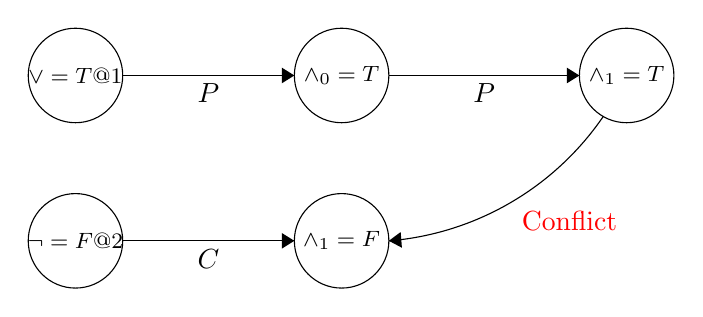
\begin{tikzpicture}[scale=0.2]
	\tikzstyle{every node}+=[inner sep=0pt]
	\draw [black] (18.4,-12.5) circle (3);
	\draw (18.4,-12.5) node {\smaller$\vee=T@1$};
	\draw [black] (35.3,-12.5) circle (3);
	\draw (35.3,-12.5) node {\smaller$\wedge_0=T$};
	\draw [black] (53.4,-12.5) circle (3);
	\draw (53.4,-12.5) node {\smaller$\wedge_1=T$};
	\draw [black] (18.4,-23) circle (3);
	\draw (18.4,-23) node {\smaller$\neg=F@2$};
	\draw [black] (35.3,-23) circle (3);
	\draw (35.3,-23) node {\smaller$\wedge_1=F$};
	\draw [black] (21.4,-12.5) -- (32.3,-12.5);
	\fill [black] (32.3,-12.5) -- (31.5,-12) -- (31.5,-13);
	\draw (26.85,-13) node [below] {$P$};
	\draw [black] (38.3,-12.5) -- (50.4,-12.5);
	\fill [black] (50.4,-12.5) -- (49.6,-12) -- (49.6,-13);
	\draw (44.35,-13) node [below] {$P$};
	\draw [black] (21.4,-23) -- (32.3,-23);
	\fill [black] (32.3,-23) -- (31.5,-22.5) -- (31.5,-23.5);
	\draw (26.85,-23.5) node [below] {$C$};
	\draw [black] (51.915,-15.103) arc (-34.40348:-85.35958:18.3);
	\fill [black] (38.3,-23) -- (39.13,-23.44) -- (39.05,-22.44);
	\draw (49.77,-21.1) node [below] {\textcolor{red}{Conflict}};
	\end{tikzpicture}
\end{center}
Dies führt nun zu einer neuen Tabelle:\\
\begin{tabular}{|c|c|c|c|c|c|c|}
	\hline 
	lvl & var & val & Reason & Clause & Stack & Comment \\ 
	\hline \hline
	1 & $\vee$ & T & Decision & - & $\vee=T@1$ & root init \\ 
	\hline 
	 & $\neg$ & T & \texttt{NoGood} & - & $\neg=T@1$ & \texttt{NoGood} flip\\ 
	\hline 
	& $\wedge_0$ & * & Parent & $\vee = T,\neg = T$ & $\wedge_0=*@1$ &  \\ 
	\hline 
	& $\wedge_1$ & * & Parent & $\wedge_0=*$ & $\wedge_1=*@1$ & don't care Vererbung \\ 
	\hline 
	& $x$ & F & Parent & $\neg = T$ & $x=F@1$ & \\ 
	\hline 
	& $y$ & * & Parent & $\wedge_0 = *$ & $y=*@1$ & \\
	\hline
	& $z$ & * & Parent & $\wedge_1 = *$ & $z=*@1$ & \\
	\hline
\end{tabular}\\\\Kein Konflikt, somit eine Menge von erfüllbaren Belegungen gefunden $$F(\texttt{False},*,*) = \texttt{True}$$
\end{document}
